\section{実験}
\label{sec:exp}
提案手法をマルウェアに適用して実験を行った.
本章では,この実験の目的,方法,結果について解説する.
また,結果に対する考察も述べる.

\subsection{実験の目的}
本研究の提案手法により得たマルウェアの実行ログから,マルウェアの挙動を明らかにできることを示す.

\subsection{実験方法}
今回,11 個の検体を用いた実験と,その 11 個の中の 1 つのマルウェアである iMatch を用いた実験の 2 種類の実験を行った.それぞれの実験方法の説明の前に\ref{expmalware} で,実験に用いたマルウェアがどのような挙動を示すかを示す.それぞれの実験については,\ref{exp1} , \ref{exp2} で詳しく説明する.

\subsubsection{実験に用いたマルウェア}
\label{expmalware}
今回の実験に用いたマルウェアの挙動を以下に示す \cite{golddream} \cite{basebridge} \cite{droiddreamlight} \cite{crazyapp} \cite{icalendar} \cite{snake} \cite{trojan} . これらのマルウェアはインターネット上のサイト \cite{malwaresite} からダウンロードした.

\begin{enumerate}
\item GoldDream
	\begin{itemize}
	\item	receiver を使うことで,SMS,電話等のシステムイベントをバックグラウンドで監視し,送信元のアドレス,電話,SMS のタイムスタンプ,電話番号をファイルに保存した後,外部のサーバへそのファイルを送信する.
	\item 外部のサーバから 4 種類のコマンドを受け取り,それを実行する.
	\begin{enumerate}
		\item SMS をバックグラウンドで送信する
		\item 電話を発信する
		\item アプリケーションをインストールまたはアンインストールする
		\item ファイルを外部のサーバへアップロードする
	\end{enumerate}
	\end{itemize}

\item basebridge
	\begin{itemize}
	\item アプリケーションのアップグレードを促すダイアログを出し.そこでアップグレードを選択すると,basebridge は com.android.battery を感染した端末にインストールする.
	\item 外部のサーバとの通信を行い,番号などが載った configuration list  をダウンロードし,この情報を基に,SMS を送信する.
	\item SMS をバックグラウンドで送信したことをユーザに気付かれないようにするために,モバイルキャリアからの課金確認の SMS をブロックする.
	\end{itemize}

\item com.tencent.qqgame
	\begin{itemize}
	\item 挙動は GoldDream と同じ
	\end{itemize}

\item Beauty Breast
	\begin{itemize}
	\item 感染した端末に電話がかかってくると,その端末の端末番号,機種名,SDK バージョン等の端末の情報を外部サーバへ送る.
	\item 新しいパッケージのインストールと,それを促すプロンプトを表示する.
	\item マルウェア自身では,上の挙動をすることはなく,ユーザの何らかの操作無しでは実行されない.
	\end{itemize}

\item Beauty Leg
	\begin{itemize}
	\item Beauty Breast と挙動は同じ.
	\end{itemize}

\item Beauty Girl
	\begin{itemize}
	\item Beauty Breast と挙動は同じ.
	\end{itemize}

\item crazy app
	\begin{itemize}
	\item 感染した端末の IMEI (端末を識別する番号) を外部サーバへ送信する.
	\item  ブラウザのブックマーク情報とブラウザの閲覧履歴をアップロードする.
	\end{itemize}
\item iCalendar
	\begin{itemize}
	\item 有料サービスに登録させるためにある番号へ SMS をバックグラウンドで送信する.
	\item SMS  を送信できたかどうかをタグとして内部で記録している.
	\item ユーザに気づかれるのを防ぐために一度しか行われない.
	\end{itemize}
	
\item iMatch
	\begin{itemize}
	\item 挙動は iCalendar と同じ.
	\end{itemize}
	
\item Snake App
	\begin{itemize}
	\item バックグラウンドで外部サーバに端末の GPS 情報を送信する.
	\item 表向きはゲームアプリケーションとして振舞っている.
	\end{itemize}
	

\item com.tencent.qq
	\begin{itemize}
	\item 感染した端末の IMEI 番号,電話番号,登録者 ID,SIM カードのシリアル番号を盗み,外部のサーバへ送信する.
	\item 過去に SMS を送った電話番号を収集する.
	\item 外部のサーバからコマンドを受け取り,以下の動作を行う
	\begin{enumerate}
		\item SMS コンテンツや URL をサーバから受け取った電話番号へ送信する.
		\item ある URL から APK ファイルをダウンロードし,それをインストールする.
		\item ブラウザにブックマークを追加する.
		\item ある URL へ誘導するポップアップを表示する.
	\end{enumerate}
	\item ログファイルに記載されている電話番号からの SMS をブロックする.
	\end{itemize}
\end{enumerate}

\subsubsection{実験 1: 11 個の検体を用いた実験}
\label{exp1}
実験 1 では\ref{expmalware} で挙げた 11 個の検体に対して,\ref{methodtop}で述べた手法を適用し.それぞれのマルウェアを実機で実行してログから挙動を解析できるかどうかを実験する.

実際にマルウェアにログコードを挿入する前の準備として,ログコードを挿入するクラスを絞り込む.
なぜこの処理が必要であるかというと,マルウェアのソースコード中の全てのクラスのメソッドにログコードを挿入してしまうと,不必要なログが大量にでてきてしまうためだ.
例えば,ゲームアプリケーションの場合,常に描画のためのメソッドが実行されている.
このようなメソッドと不正を動きをしているメソッドのログが混ざって出力されてしまうと,解析が非常に行いづらい.
マルウェアのソースコード (Java クラスファイル) を探索し,"install", "download", "SMS", "remote" などのマルウェアの代表的な挙動を表す単語を含むメソッドのクラスを不正な動きをするクラスとみなし,コードを挿入するクラスとする.

コードを挿入するクラスを決定した後,そのクラスのメソッドの先頭にログコードを挿入した.
ログコードが挿入されたマルウェアを Nexus 5 (Android 4.4.4) にインストールした後,手動でそれぞれのマルウェアを起動した.

\subsubsection{実験 2: SMS  を送るマルウェアの実験}
\label{exp2}
実験 2 では,\ref{methodtop}, \ref{methodcalls}の 2 つの手法を適用する.
この実験では SMS を送るマルウェアである iMatch に対して行った.
実験 1 と同様にコードを挿入するクラスを決定した後に,そのクラスのメソッドに対して,メソッド呼び出しの前後にログコードを挿入した.
さらに,\ref{private}で説明した方法を用いて,一部の private メソッドにもコードを挿入した.
その後,メソッドの先頭へログコードを挿入した.
これも実験 1 と同じ操作である.
そして,ログコードを挿入した iMatch を Nexus 5 (Android 4.4.4) にインストールして,これを起動した.

\subsection{実験結果}
\subsubsection{実験 1 の結果}
11 個中,8 個のマルウェアからログを得ることができた.
その 8 個の中の 5 個では,不正な動きを示すログを得ることができた.
これら 5 つの結果を以下に示すと同時に,得られた結果と\ref{expmalware}との比較を述べる.
また,その他の 3 つのマルウェアについて,不正な挙動のログが得られなかった原因を考察する.

\begin{enumerate}
\item GoldDream \mbox{}\\
	\ \ 3 種類のメソッドのログを得ることができた.
	図\ref{zjservicereceive}, 図\ref{zjservicegetkey},図\ref{zjserviceuseragent}は,この実験で GoldDream から得られたログである.
	
	\ \ 図\ref{zjservicereceive}の onReceive は端末を起動したときに実行された.
	このメソッドの第2引数は Intent といい,アプリケーション間のデータのやりとりや連携を行うための Android API のオブジェクトである.
	"BOOT\_COMPLETED" は端末の起動が完了したことを表し,”cmp" の値は起動されるアプリケーションのパッケージ名を表している.
	端末が起動したときに ”BOOT\_COMPLETED” というイベントが Android OS 内で発生する.
	つまり,このログから,端末が起動したイベントを検知してマルウェア自身を起動していることがわかる.
	
	\ \ 図\ref{zjservicegetkey}のgetKeyNode は一度に 10 回動時に実行され,これが定期的に行われる.
	引数の中身は,"ms", "ms\_v", "rtt", "rtt\_v", "uwf", "uwf\_v" など,何らかの略称を表しているが,これらが何を表しているかがよくわからなかった.
	そのため,このメソッドが何をしようとしているかが推測できなかった.
	
	\ \ 図\ref{zjserviceuseragent}の getUserAgent は getKeyNode と同時に実行されるが,getKeyNode のように必ずしも毎回実行されるわけではない.
	このメソッドは引数がなかったため,このメソッド内で何が起こっているのかがわからなかった.
	
	\ \ この結果からこのマルウェアが receiver を用いてシステムイベントを監視し,何らかの情報を収集しようとしていることがわかった.
	しかし,外部との通信を行っている挙動は確認できなかった.
	
\item com.tencent.qqgame \mbox{}\\
	\ \ 2 種類のメソッド,getCommunicator, isConnected のログを得ることができた.
	この結果を図\ref{qqgame} に示す.
	この 2 つのメソッドはこのアプリケーションの画面からホーム画面へ戻る操作をしたときに,この 2 つのメソッドが同時に実行される.
	getCommunnicator メソッドにより, 何らかの通信コネクションを表すオブジェクトを取得していることがわかる.
	また,図\ref{qqgame}の 3, 4 行目から,isConnected メソッドは SocketCommunicator クラスのメソッドであることが読み取れる.
	よって,このマルウェアが外部の通信を試みようとしていて,このメソッドで通信が確立されているかを確かめていることがわかる.
	
	\ \ 今回の実験ではシステムイベントを監視している挙動のログを得ることができなかった.
	この原因の一つは.この実験で用いた Nexus 5 には SIM カードが入っていないためである.
	そのため,今回の実験環境は,このマルウェアが監視している電話の着信,SMS の受信などのイベントが発生しない環境であった.
	つまり,マルウェアが電話や SMS の情報を収集しようとしてもその情報がない状況だった.
	
\item iCalendar \mbox{}\\
	\ \ 得られたログの結果を図\ref{calendar}に示す.
	SMS を送信していることを示すメソッド sendSms のログを得ることができた.
	このメソッドはアプリケーションが起動した状態で画面を 5 回タップすると実行される.
	このメソッドが実行された時は画面には何も表示されない.
	何度かインストールを行うことで,このメソッドがインストール後一回のみ実行されることも確認した.
	
	\ \ しかし,SMS が送られたかどうかを記録する挙動のログは今回の実験では得ることができなかった.
	Android 端末だけでなくモバイル端末は SIM カードがないとSMS を送信することができない.
	実験で使用した Nexus 5 には SIM カードが挿入されていなかったために SMS が送信できなかった.
	そのため,送信ができなかったという記録をする挙動をしてもよいはずである.
	この動作をするクラスにログを挿入していなかったため,もしくは Android API を用いて記録したためにログとして出てこなかったことが考えられる.
	
\item iMatch \mbox{}\\
	\ \ 図\ref{imatch} がこの実験で得られたログである.
	SMS 送信を示すメソッド,sendSms を確認できた.
	このメソッドはこのマルウェアを起動すると実行され,この時,端末の画面には何も変化はなかった.
	iCalendar とは異なり,このメソッドが実行されるのは一度だけではないことがわかった.
	インストールを一度しかしていなくても,何度か起動することで図\ref{imatch}と同様のログが何回も出力されたからである.
	
	\ \ iCalendar の場合と同様に,SMS を送信したかどうか記録している挙動のログを出力させることはできなかった.
	この理由としては,iCalendar と同じであると考えられる.
	iMatch は iCalendar と同じ作成者なので \cite{icalendar},この 2 つのマルウェアがSMS を送信する手段は似ていると考えられるためだ .
	
\item com.tencent.qq \mbox{}\\
	\ \ 図\ref{qqauthentication}と図\ref{qqreceive}のログを得ることができた.
	
	\ \ 図\ref{qqauthentication}の getCodeByURL では引数に URL をとっている.
	よって,この URL からコードを取得することがわかる.
	このメソッドはマルウェアの起動に関係なく,15 分おきに 2 回実行される.
	2 番目の int 型の引数は 1 回目と 2 回目で異なる値である.
	1 回目は 0 で,2 回目は 1 である.第一引数の URL は常に同じであった.
	
	\ \ このマルウェアをインストールした後に,端末を再起動すると,最初に SMS を送る確認をするダイアログが現れる.
	図\ref{dialog}はそのダイアログである.
	このダイアログで "Send" を選択すると,onReceive が実行され,図\ref{qqreceive}のログが出力された.
	このダイアログは端末を起動する度に毎回現れる.
	このメソッドの引数の Intent は他のアプリケーションに SMS を送信するアクションを行うように指示している.
	つまり,このメソッドで SMS を送信することがわかる.
	
	\ \ この実験では,外部へメッセージなどを送信しようとしているログ,またブックマークを追加するログを出力することはできなかった.
	実験で用いた Nexus 5 のブラウザである Googl Chrome のブックマークを確認したところ,このマルウェアによってブックマークが追加されていなかった.
	外部からコマンドを受け取ろうとしているメソッドのログを得ることはできたが,実際にコマンドを受け取ったたかどうかまではこの実験の結果からは分からない.
\end{enumerate}


\begin{figure}[t]
\begin{center}
\graphicspath{{./epsfiles/}}
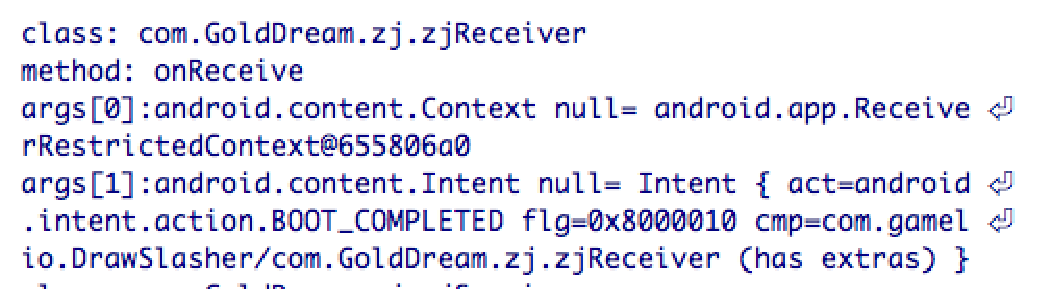
\includegraphics[scale=0.5]{onreceivezjservice.eps}
\end{center}
\caption{GoldDream の onReceive のログ}
\label{zjservicereceive}
\end{figure}

\begin{figure}[t]
\begin{center}
\graphicspath{{./epsfiles/}}
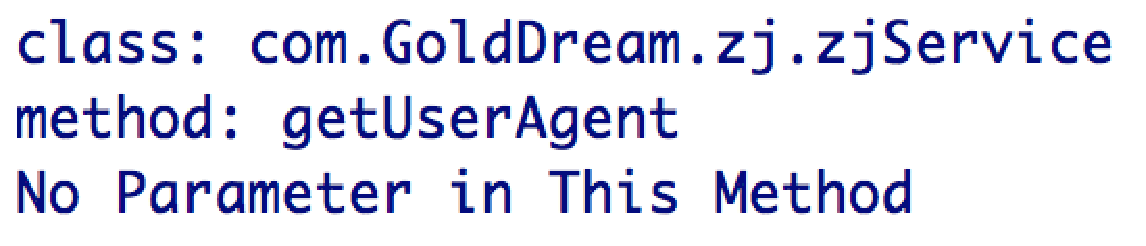
\includegraphics[scale=0.3]{getuseragentzjservice.eps}
\end{center}
\caption{GoldDream の getUserAgent のログ}
\label{zjserviceuseragent}
\end{figure}

\begin{figure}[t]
\begin{center}
\graphicspath{{./epsfiles/}}
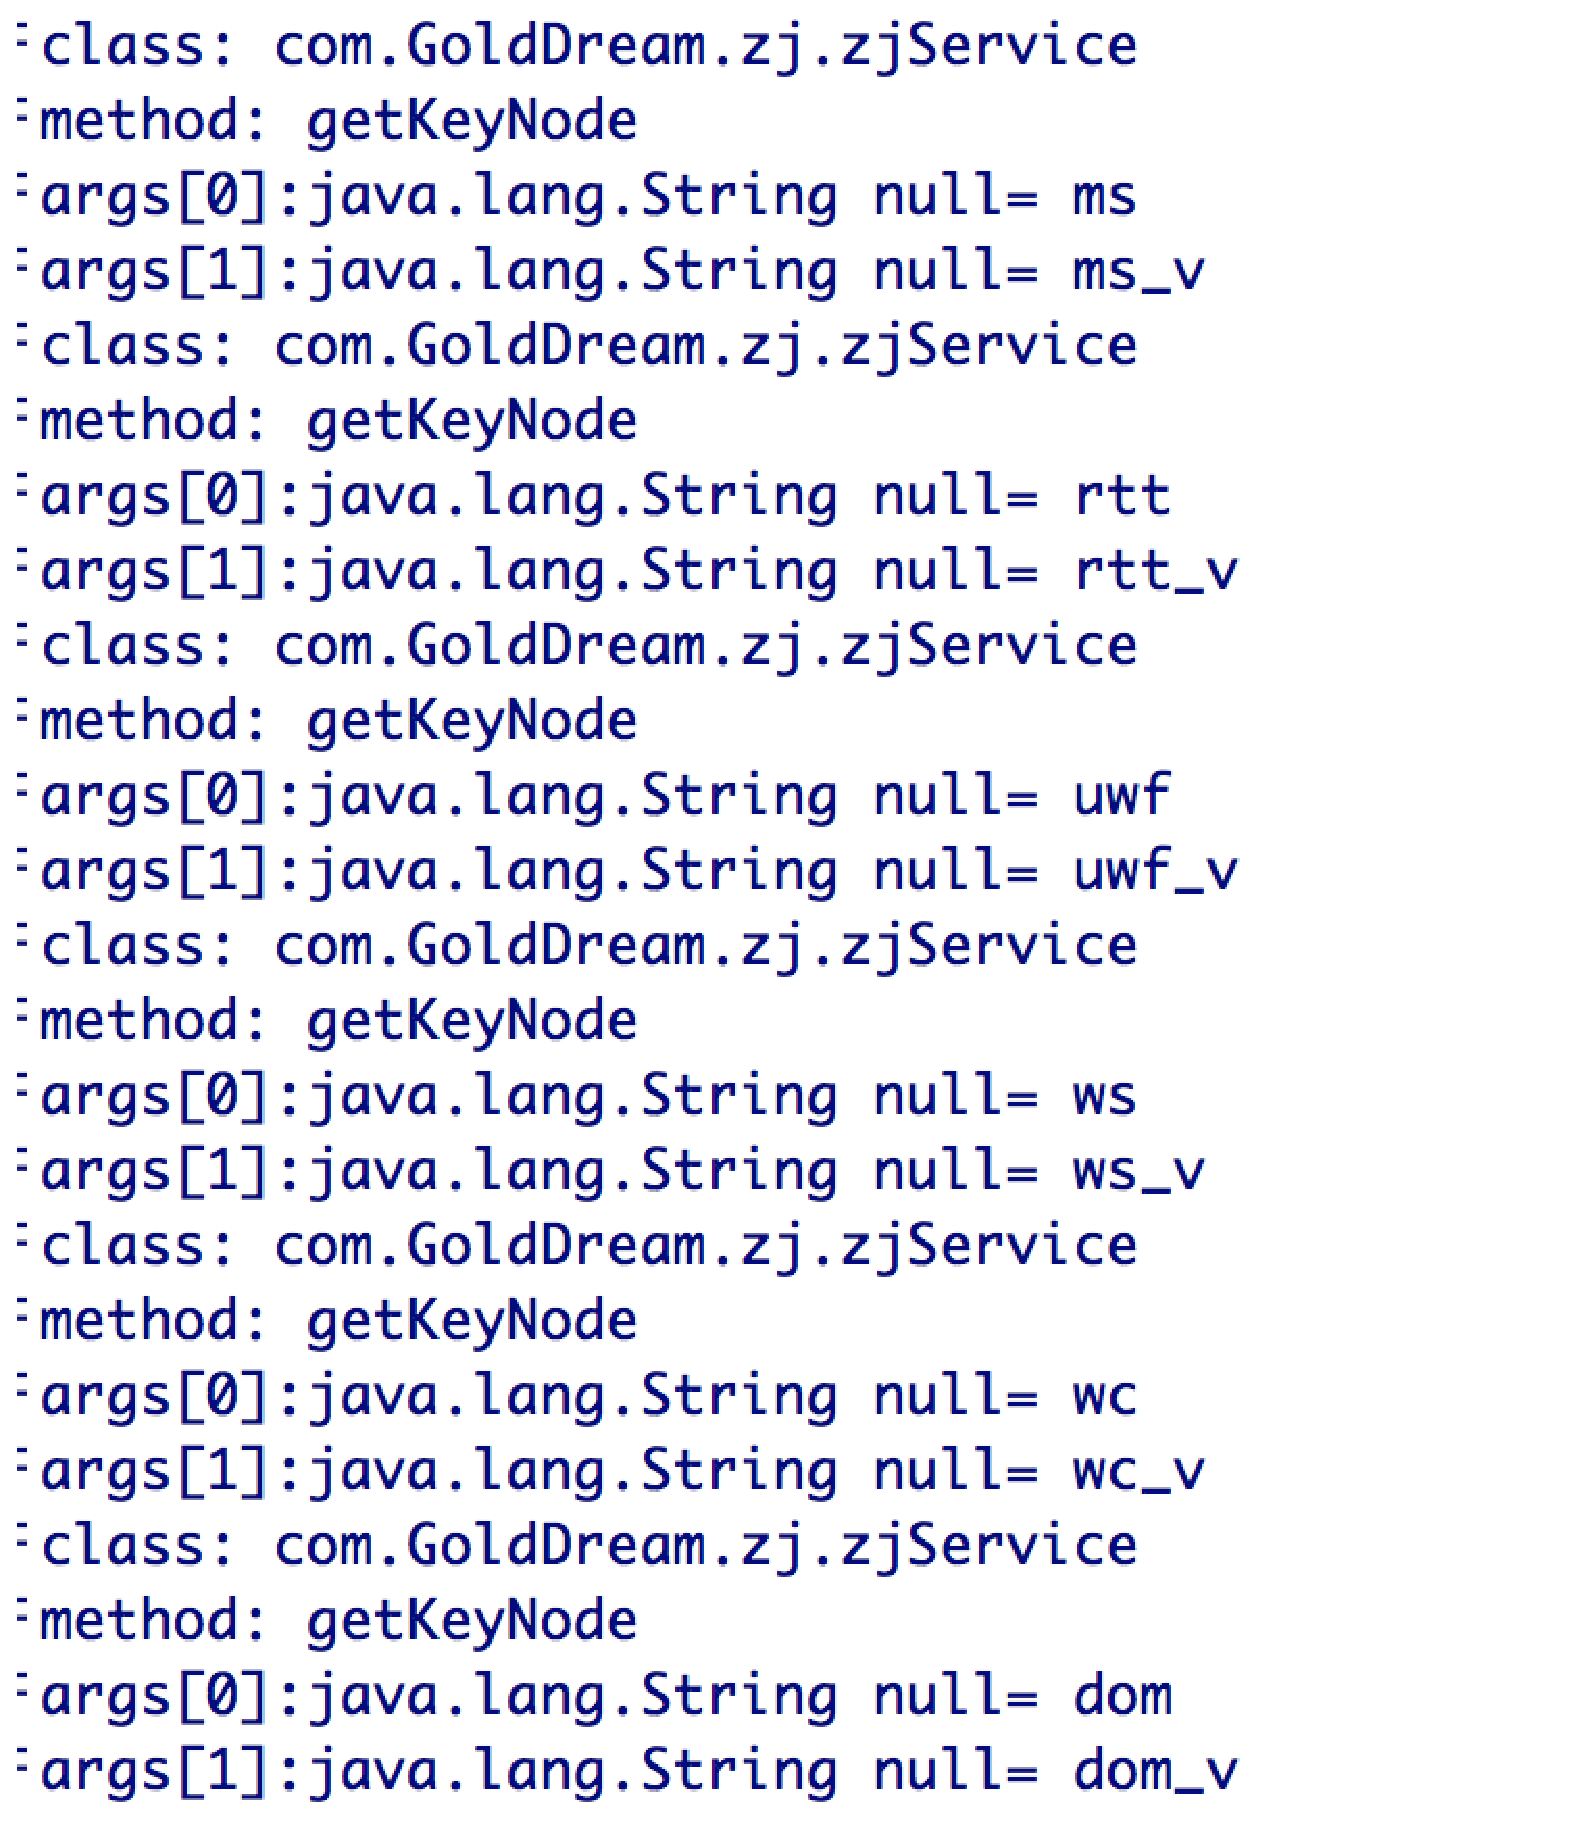
\includegraphics[scale=0.2]{getkeynodezjservice.eps}
\end{center}
\caption{GoldDream の getKeyNode のログ}
\label{zjservicegetkey}
\end{figure}

\begin{figure}[t]
\begin{center}
\graphicspath{{./epsfiles/}}
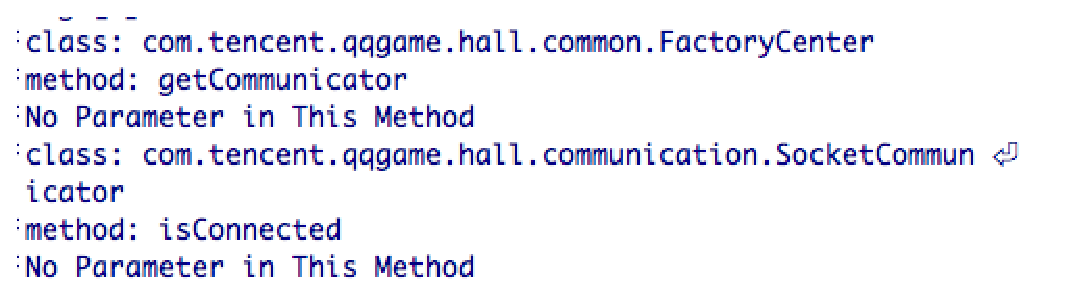
\includegraphics[scale=0.45]{qqgame.eps}
\end{center}
\caption{com.tencent.qqgame のメソッドのログ}
\label{qqgame}
\end{figure}

\begin{figure}[t]
\begin{center}
\graphicspath{{./epsfiles/}}
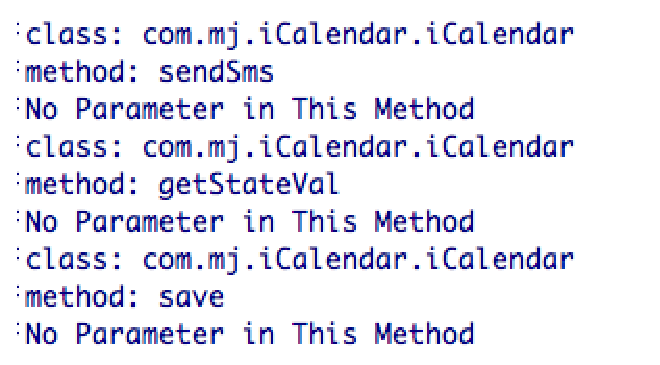
\includegraphics[scale=0.45]{icalendar1.eps}
\end{center}
\caption{iCalendar のメソッドのログ}
\label{calendar}
\end{figure}

\begin{figure}[t]
\begin{center}
\graphicspath{{./epsfiles/}}
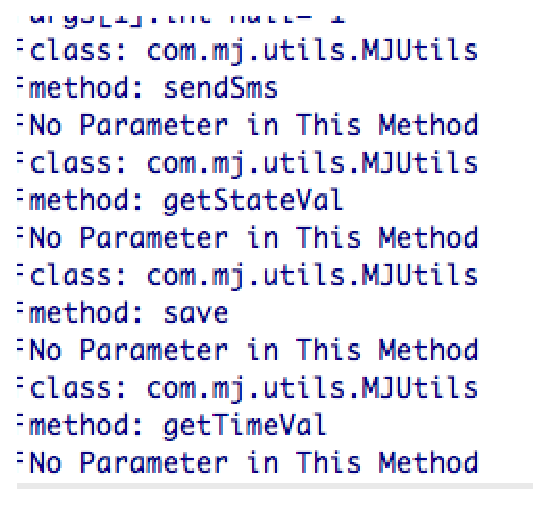
\includegraphics[scale=0.45]{imatch_sendsms.eps}
\end{center}
\caption{iMatch のメソッドのログ}
\label{imatch}
\end{figure}

\begin{figure}[t]
\begin{center}
\graphicspath{{./epsfiles/}}
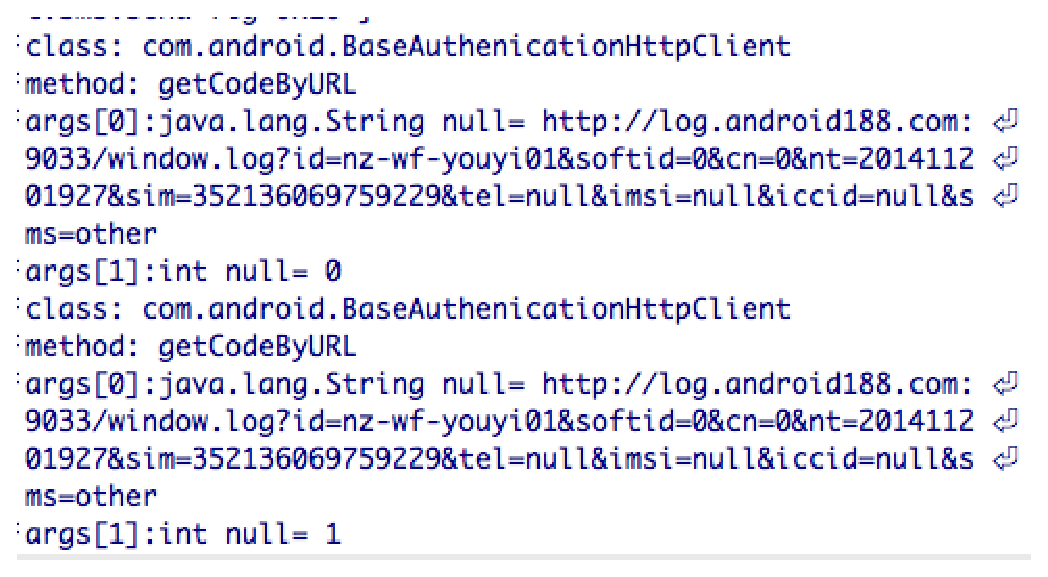
\includegraphics[scale=0.5]{baseauthentication_qq.eps}
\end{center}
\caption{com.tencent.qq の getCodeByURL のログ}
\label{qqauthentication}
\end{figure}


\begin{figure}[t]
\begin{center}
\graphicspath{{./epsfiles/}}
\includegraphics[scale=0.1]{nexus_qq_dialog.eps}
\end{center}
\caption{com.tencent.qq のダイアログ}
\label{dialog}
\end{figure}

\begin{figure}[t]
\begin{center}
\graphicspath{{./epsfiles/}}
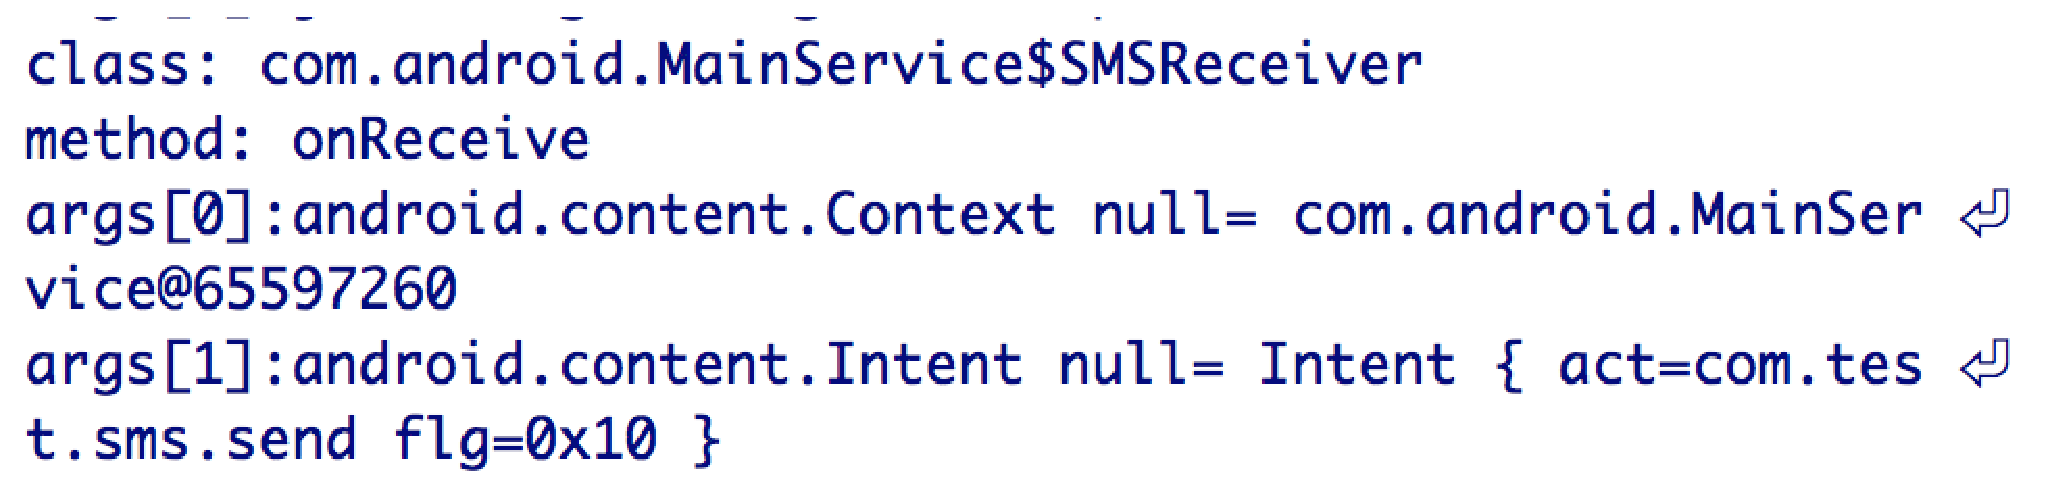
\includegraphics[scale=0.3]{SmsReceiver_qq.eps}
\end{center}
\caption{com.tencent.qqの onReceive のログ}
\label{qqreceive}
\end{figure}

Beauty Leg, Beauty Breast, Beauty Girl の 3 個のマルウェアからは,ログを得ることはできたが,図\ref{leg}のようにメソッド名が一文字のアルファベットであるためメソッドの内容を推測することができなかった,また,得られたメソッドのログの引数の中身を見ても,挙動を特定することができなかった.なお,図\ref{leg}の 1 つ目 (onCreate) と 3 つ目のメソッド (onStart) はそれぞれ android.app.Activity クラスのメソッドであり,全ての Android アプリケーションは Activity クラスをオーバーライドしたクラスを持つ.そのため,onCreate, onStart はこのマルウェアの特有のメソッドではない.

不正な動きのログを得られなかったのは,これらのマルウェアのトリガーを再現できなかったためである.\ref{expmalware} で述べたように,この 3 つのマルウェアは電話の着信で起動する.モバイル端末は SIM カードがないと電話の発着信ができない.実験を行った Nexus 5 は SIM カードを挿入していなかったため,電話機能をもっていなかった.そのため,不正な振る舞いをするコードを実行することができなかった.

\begin{figure}[t]
\begin{center}
\graphicspath{{./epsfiles/}}
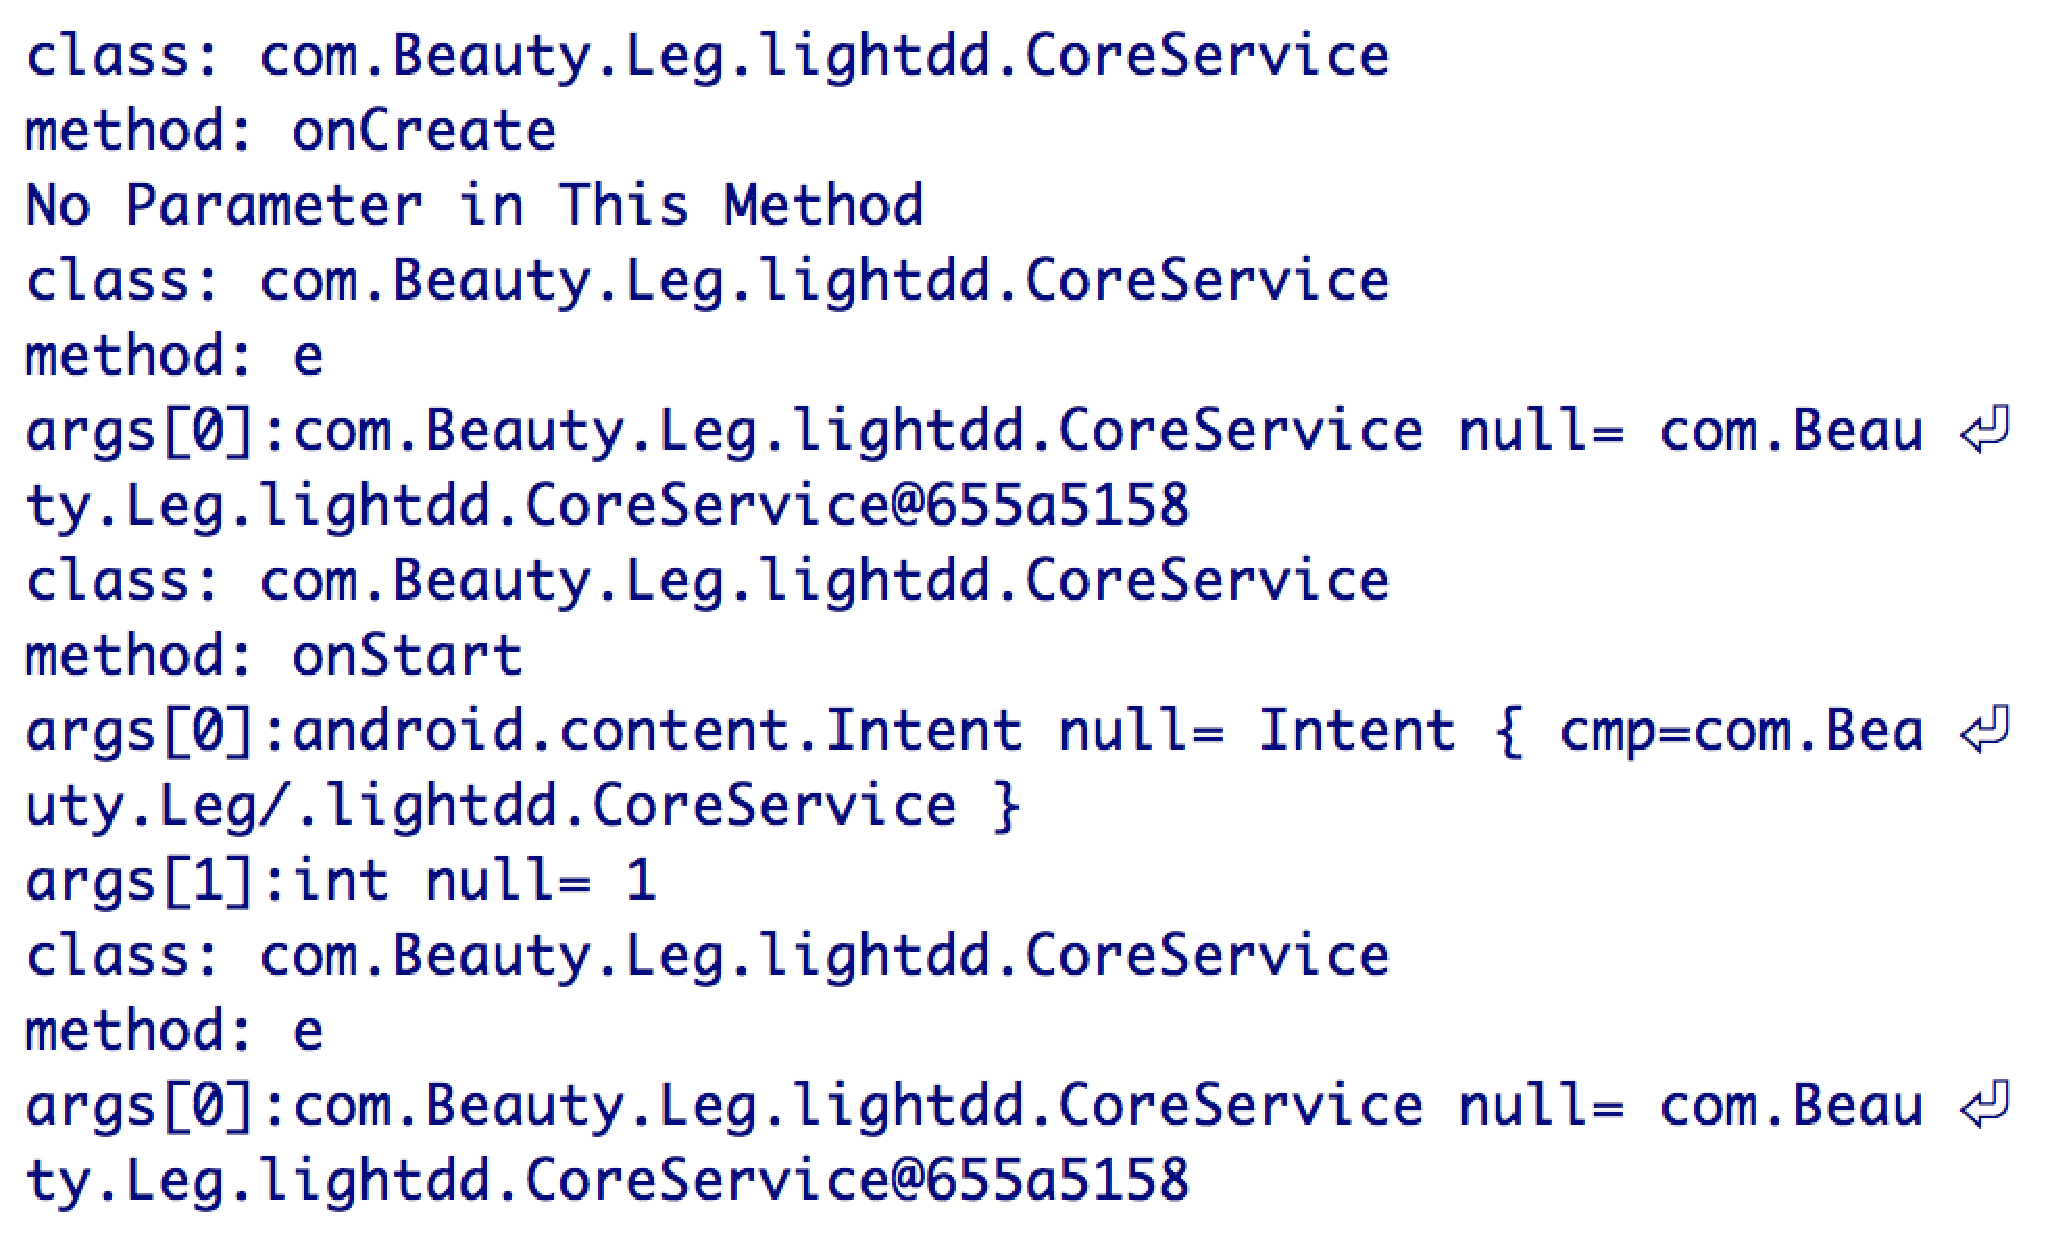
\includegraphics[scale=0.25]{beautyleg2.eps}
\end{center}
\caption{Beauty Leg のログ}
\label{leg}
\end{figure}

その他のマルウェアはログコードを挿入したにも関わらず,ログを得ることができなかった.その理由として,3 つ考えられる.ひとつはログコードを挿入した部分が少なかったこととである.図\ref{leg}のように,Beauty Leg などのアプリケーションは実際にメソッド名を変えている.よって,マルウェア作成者が解析を困難にするためにメソッド名を変えたことは十分に考えられる.メソッド名を変えられてしまうと怪しい動きを行うメソッドを探すのはとても難しい.また.今回の実験では,キーワードに基づいてメソッドを検索し,コードを挿入するクラスを決定した.そして,キーワードがメソッド名の一部だった場合,不正な動きをするクラスであると判定した.そのため,不正な振る舞いをするメソッドが存在したとしても,そのメソッドに使われている単語を推測できないとそのクラスにコードを挿入することができない.\ref{exp1}で挙げたマルウェアの代表的な挙動を表すキーワードが十分でなかったために,マルウェアの不正な動きのログを得ることができなかった可能性はある.

また,外部サーバからのコマンドを受け取らなかったために,不正な動きそのものをしなかった可能性もある,この実験で用いたマルウェアは新しいものではなく,これらのマルウェアの APK ファイルの多くは 2011 年にアップロードされたものであった\cite{malwaresite}.さらに,実験を行った時点 (2014 年 11,12 月) でこのマルウェアは解析されていた.マルウェア作成者は解析されたことに気づいて外部サーバの URL を変えたり,外部サーバを停止させる等の対策をしたために,これらのマルウェアを動かしても,外部サーバと実際に通信を行うログを得ることができなかったと考えている.

最後の原因として,一般的なメソッド,たとえば onCreate の中で不正な動きをしている可能性がある. この実験では,onCreate をはじめとする,どの Android アプリケーションも持っているメソッドに対してコードを挿入しなかった.\ref{methodtop}の手法では,メソッド名とそのクラス名,さらに引数の情報がわかるが,メソッド内で何が行われたまでは分からないためである.このようなメソッドの中で不正な動きをするコードが書かれていることは十分に考えられる.


ログを得ることができた 5 つのマルウェアも \ref{expmalware}で述べた挙動と比べると十分なものではない.上で述べた 3 つの理由はこの 5 つのマルウェアにも当てはまるからである.これらのマルウェアには,ログコードを挿入していない部分がまだまだ多数存在する.そのため,実際に実行された全てのメソッドにコードを挿入していない.また,外部サーバが実際に動作していなかったり ,全ての Android アプリケーションに共通なメソッド内で何か不正なコードが書かれているかもしれない.そこで,実験 2 ではメソッド内のメソッド呼び出しをログとして出力することで,メソッド内の様子を明らかにする.


\subsubsection{実験 2 の結果}
この実験で得られた 2 つのクラス (com.mj.imatch.IMatch, com.mj.utils.MJUtils) のログのテキストの一部を以下の図に示す\ref{imatchlog} \ref{mjutilslog1} \ref{mjutilslog2}.
なお,紙面の都合上,ログの一部の情報を除いた形で載せている.
このログのテキストを得るために\ref{splitscript}のプログラムを用いた.

図\ref{imatchlog}の28 行目より,IMatch クラスの onCreate が sendSms を実行していることを示している.
onCreate メソッドがあるということはこのクラスは android.app.Activity クラスの子クラスということになる.
図\ref{imatchmanif}は iMatch の AndroidManifest.xml である.
図\ref{imatchmanif} の 5 から10 行目に,IMatch クラスについて記されている.
7 行目は,iMatch が起動したときに IMatch クラスが最初に表示される activity であるということを意味している.
Android の activity は図\ref{activity}に示すような状態遷移を行う\cite{activity}.
activity クラスのオブジェクトは生成されると, 最初に onCreate が実行される.
つまり,iMatch が起動されると最初に IMatch クラスの onCreate が実行され,その中で sendSms が呼び出される.

\ref{private}の手法を適用するためにまず sendSms の中にどのメソッドがあるかを調べた.
図\ref{mjutilslog1}のログから,sendSms の中で sendCM, sendCM1,sendCM2, sendUC が実行されていることがわかる.
図\ref{mjutilslog1}では,この 4 つのメソッドの前後のログは出力されているが,引数の中身のログは出力されていない.
そのため,これらは private メソッドである.
また,\ref{replacement}で述べたように,呼び出されるメソッドのクラスの情報もこのログからわかる.
よって,この 4 つのメソッドは com.mj.utils.MJUtils のメソッドであることもわかった.
先ほども述べたように,図\ref{imatchlog}, 図\ref{mjutilslog1},  図\ref{mjutilslog2}では,呼び出されるメソッドのクラスが記されている部分は除いてある.
private メソッドの名前とそのクラスがわかったので,\ref{private}の手法を適用し,他の条件は同じにして,iMatch をもう一度インストールし,得られたログのテキスト\ref{mjutilslog2}を得た.
\ref{private}の手法を適用したのは,sendCM, sendCM1, sendCM2, sendUC の 4 つのみである.


図\ref{mjutilslog2}は,iMatch が SMS を送るために sendTextMessage というメソッドを用いていることを示している.
このメソッドのクラスは android.telephony.gsm.SmsManager であり,これは Android API の 1 つである\cite{smsmanager}.sendTextMessage は文字通り SMS を送るメソッドである.このメソッドの引数は以下に示すように 5 つある.MJUtils の sendSms の中では sendTextMessage が 4 回実行されている.しかし,このメソッドは Android API であるため,sendTextMessage の中にコードを挿入することができない.
そのため,sendTextMessage の引数についての情報を得ることができなかった.
よって,それぞれのメソッドがどんなメッセージをどの番号へ SMS を送信しているかはわからなかった.

\begin{itembox}[c]{SmsManager.sendTextMessage}
public final void sendTextMessage(String destAddress, String srcAddress, String text, PendingIntent sentIntent, PendingIntent deliveryIntent)
\end{itembox}

\begin{figure}[t]
\begin{center}
\graphicspath{{./epsfiles/}}
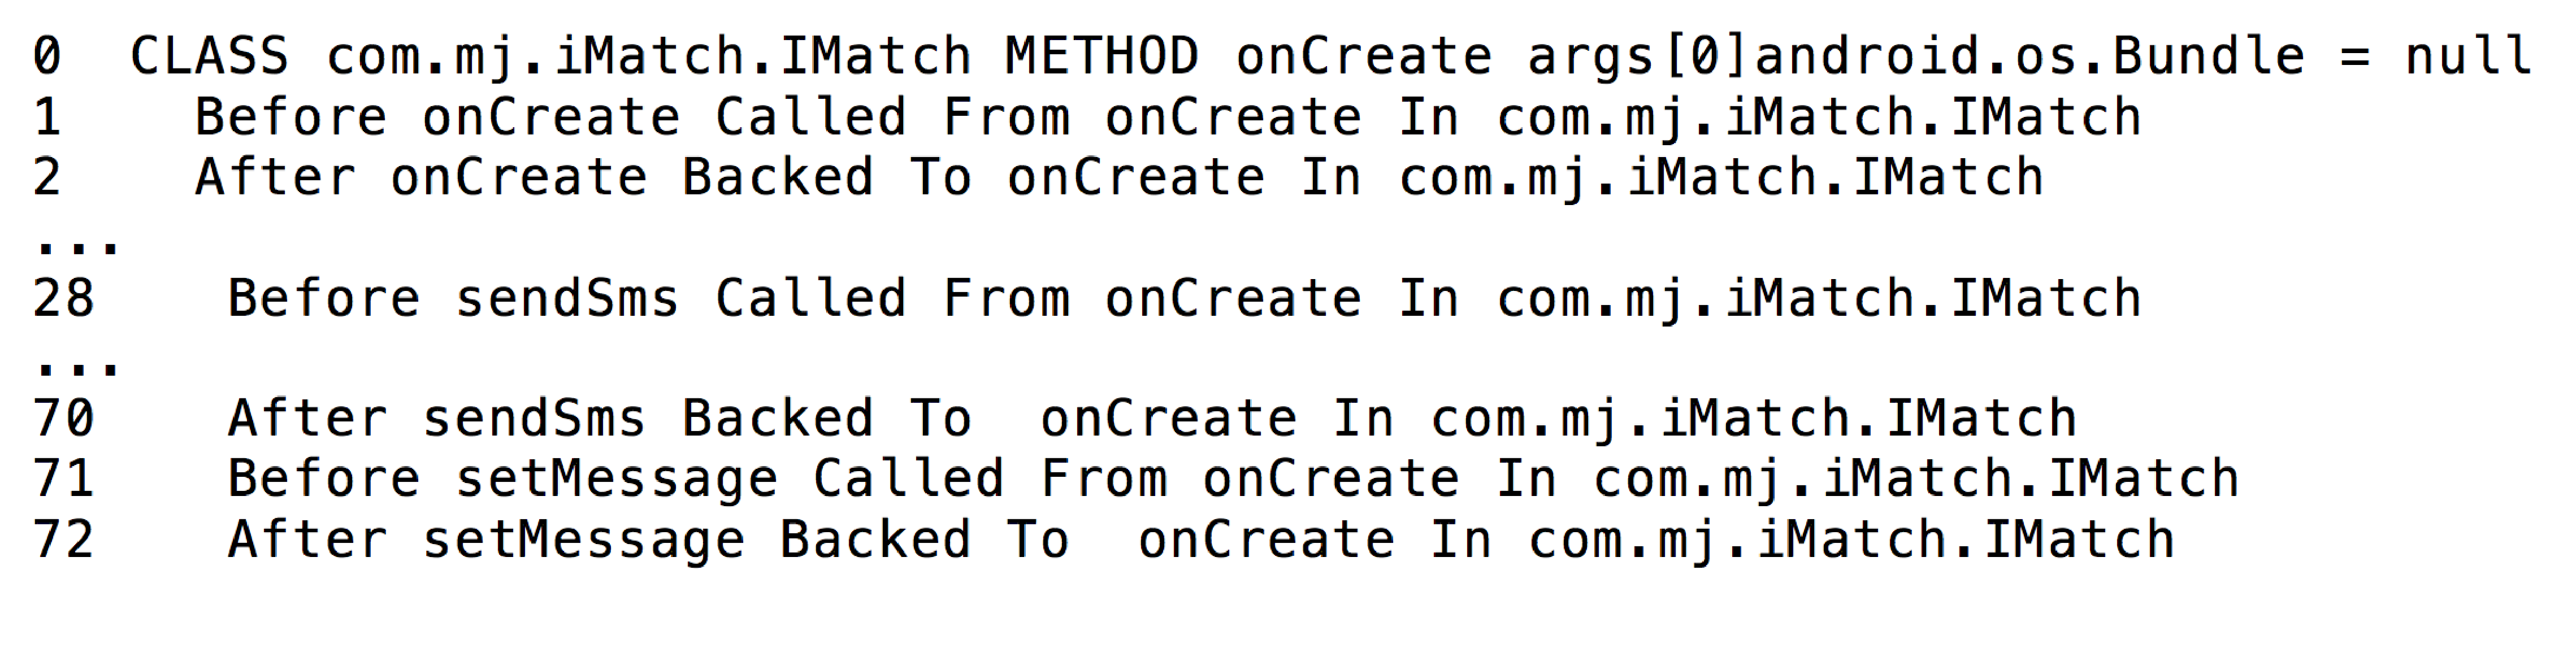
\includegraphics[scale=0.2]{logtext1.eps}
\end{center}
\caption{com.mj.iMatch.IMatch のログのテキストの一部 のログ}
\label{imatchlog}
\end{figure}


\begin{figure}[t]
\begin{center}
\graphicspath{{./epsfiles/}}
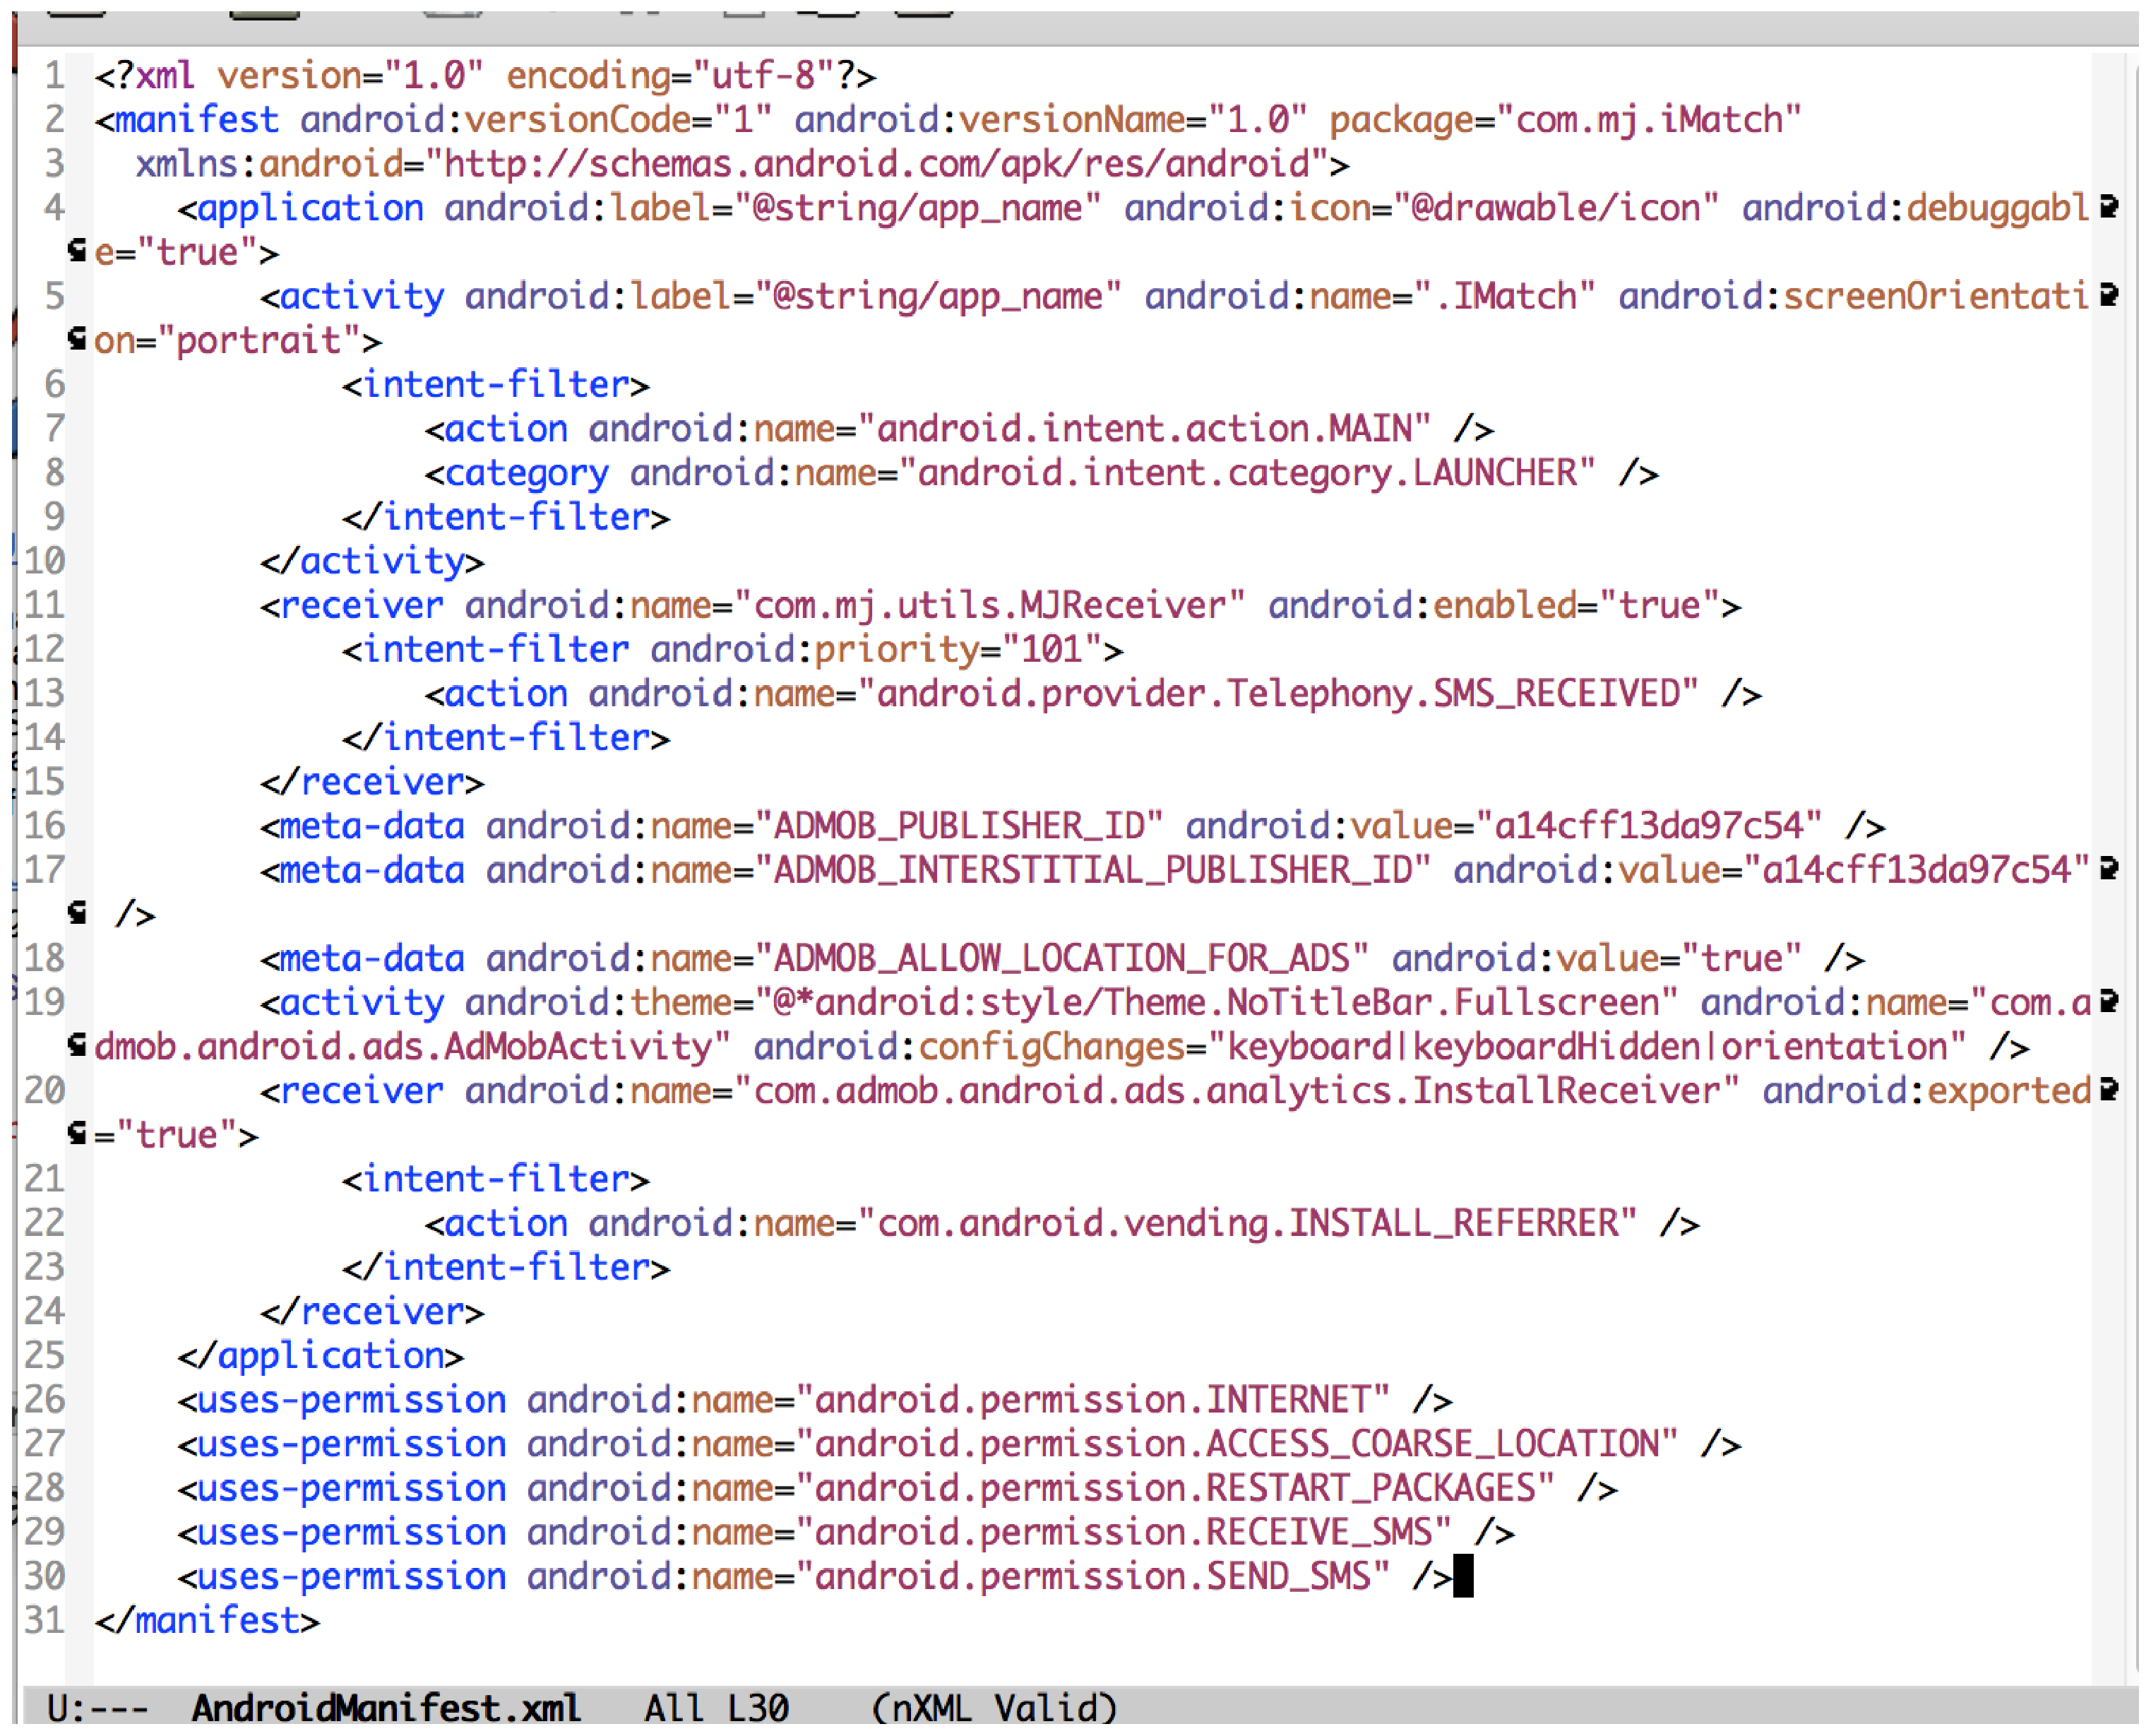
\includegraphics[scale=0.2]{imatchmanifest.eps}
\end{center}
\caption{iMatch の AndroidManifest.xml}
\label{imatchmanif}
\end{figure}

\begin{figure}[t]
\begin{center}
\graphicspath{{./epsfiles/}}
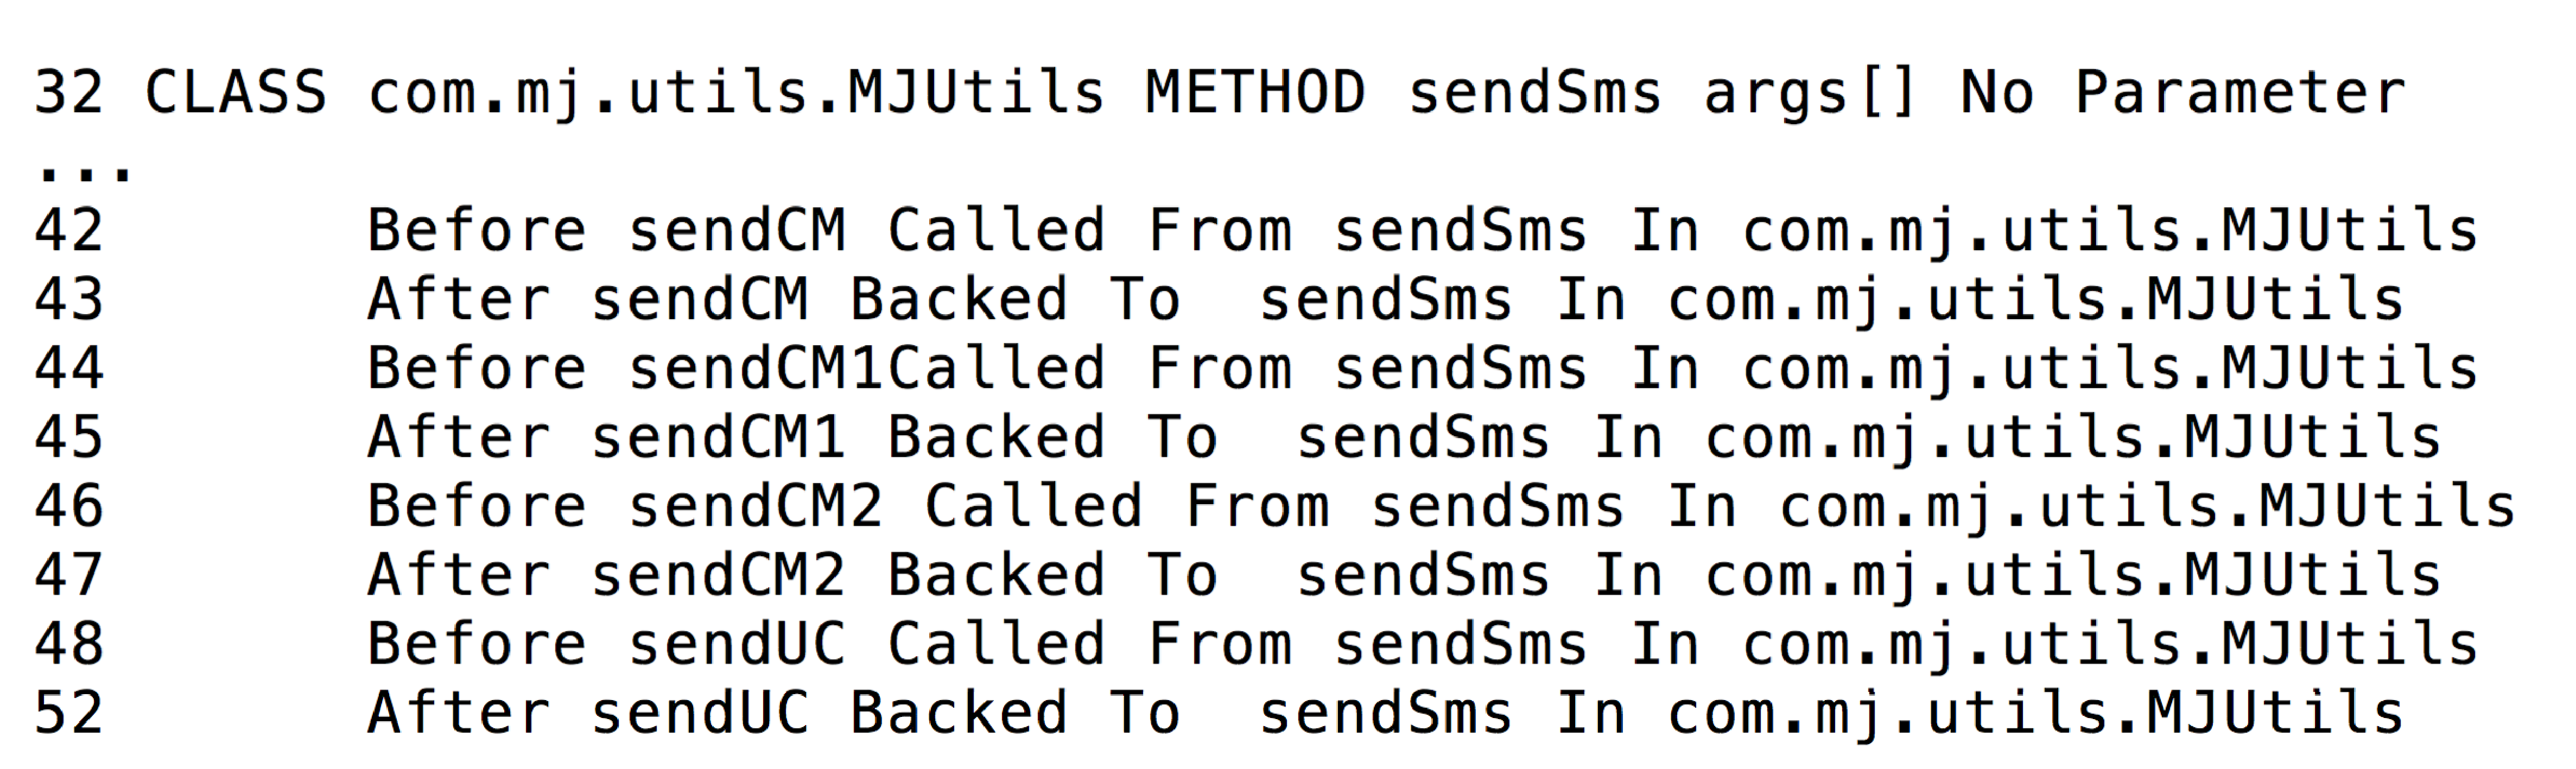
\includegraphics[scale=0.15]{mjutilslog1.eps}
\end{center}
\caption{\ref{private} の手法適用前のcom.mj.utils.MJUtils のログのテキストの一部}
\label{mjutilslog1}
\end{figure}

\begin{figure}[t]
\begin{center}
\graphicspath{{./epsfiles/}}
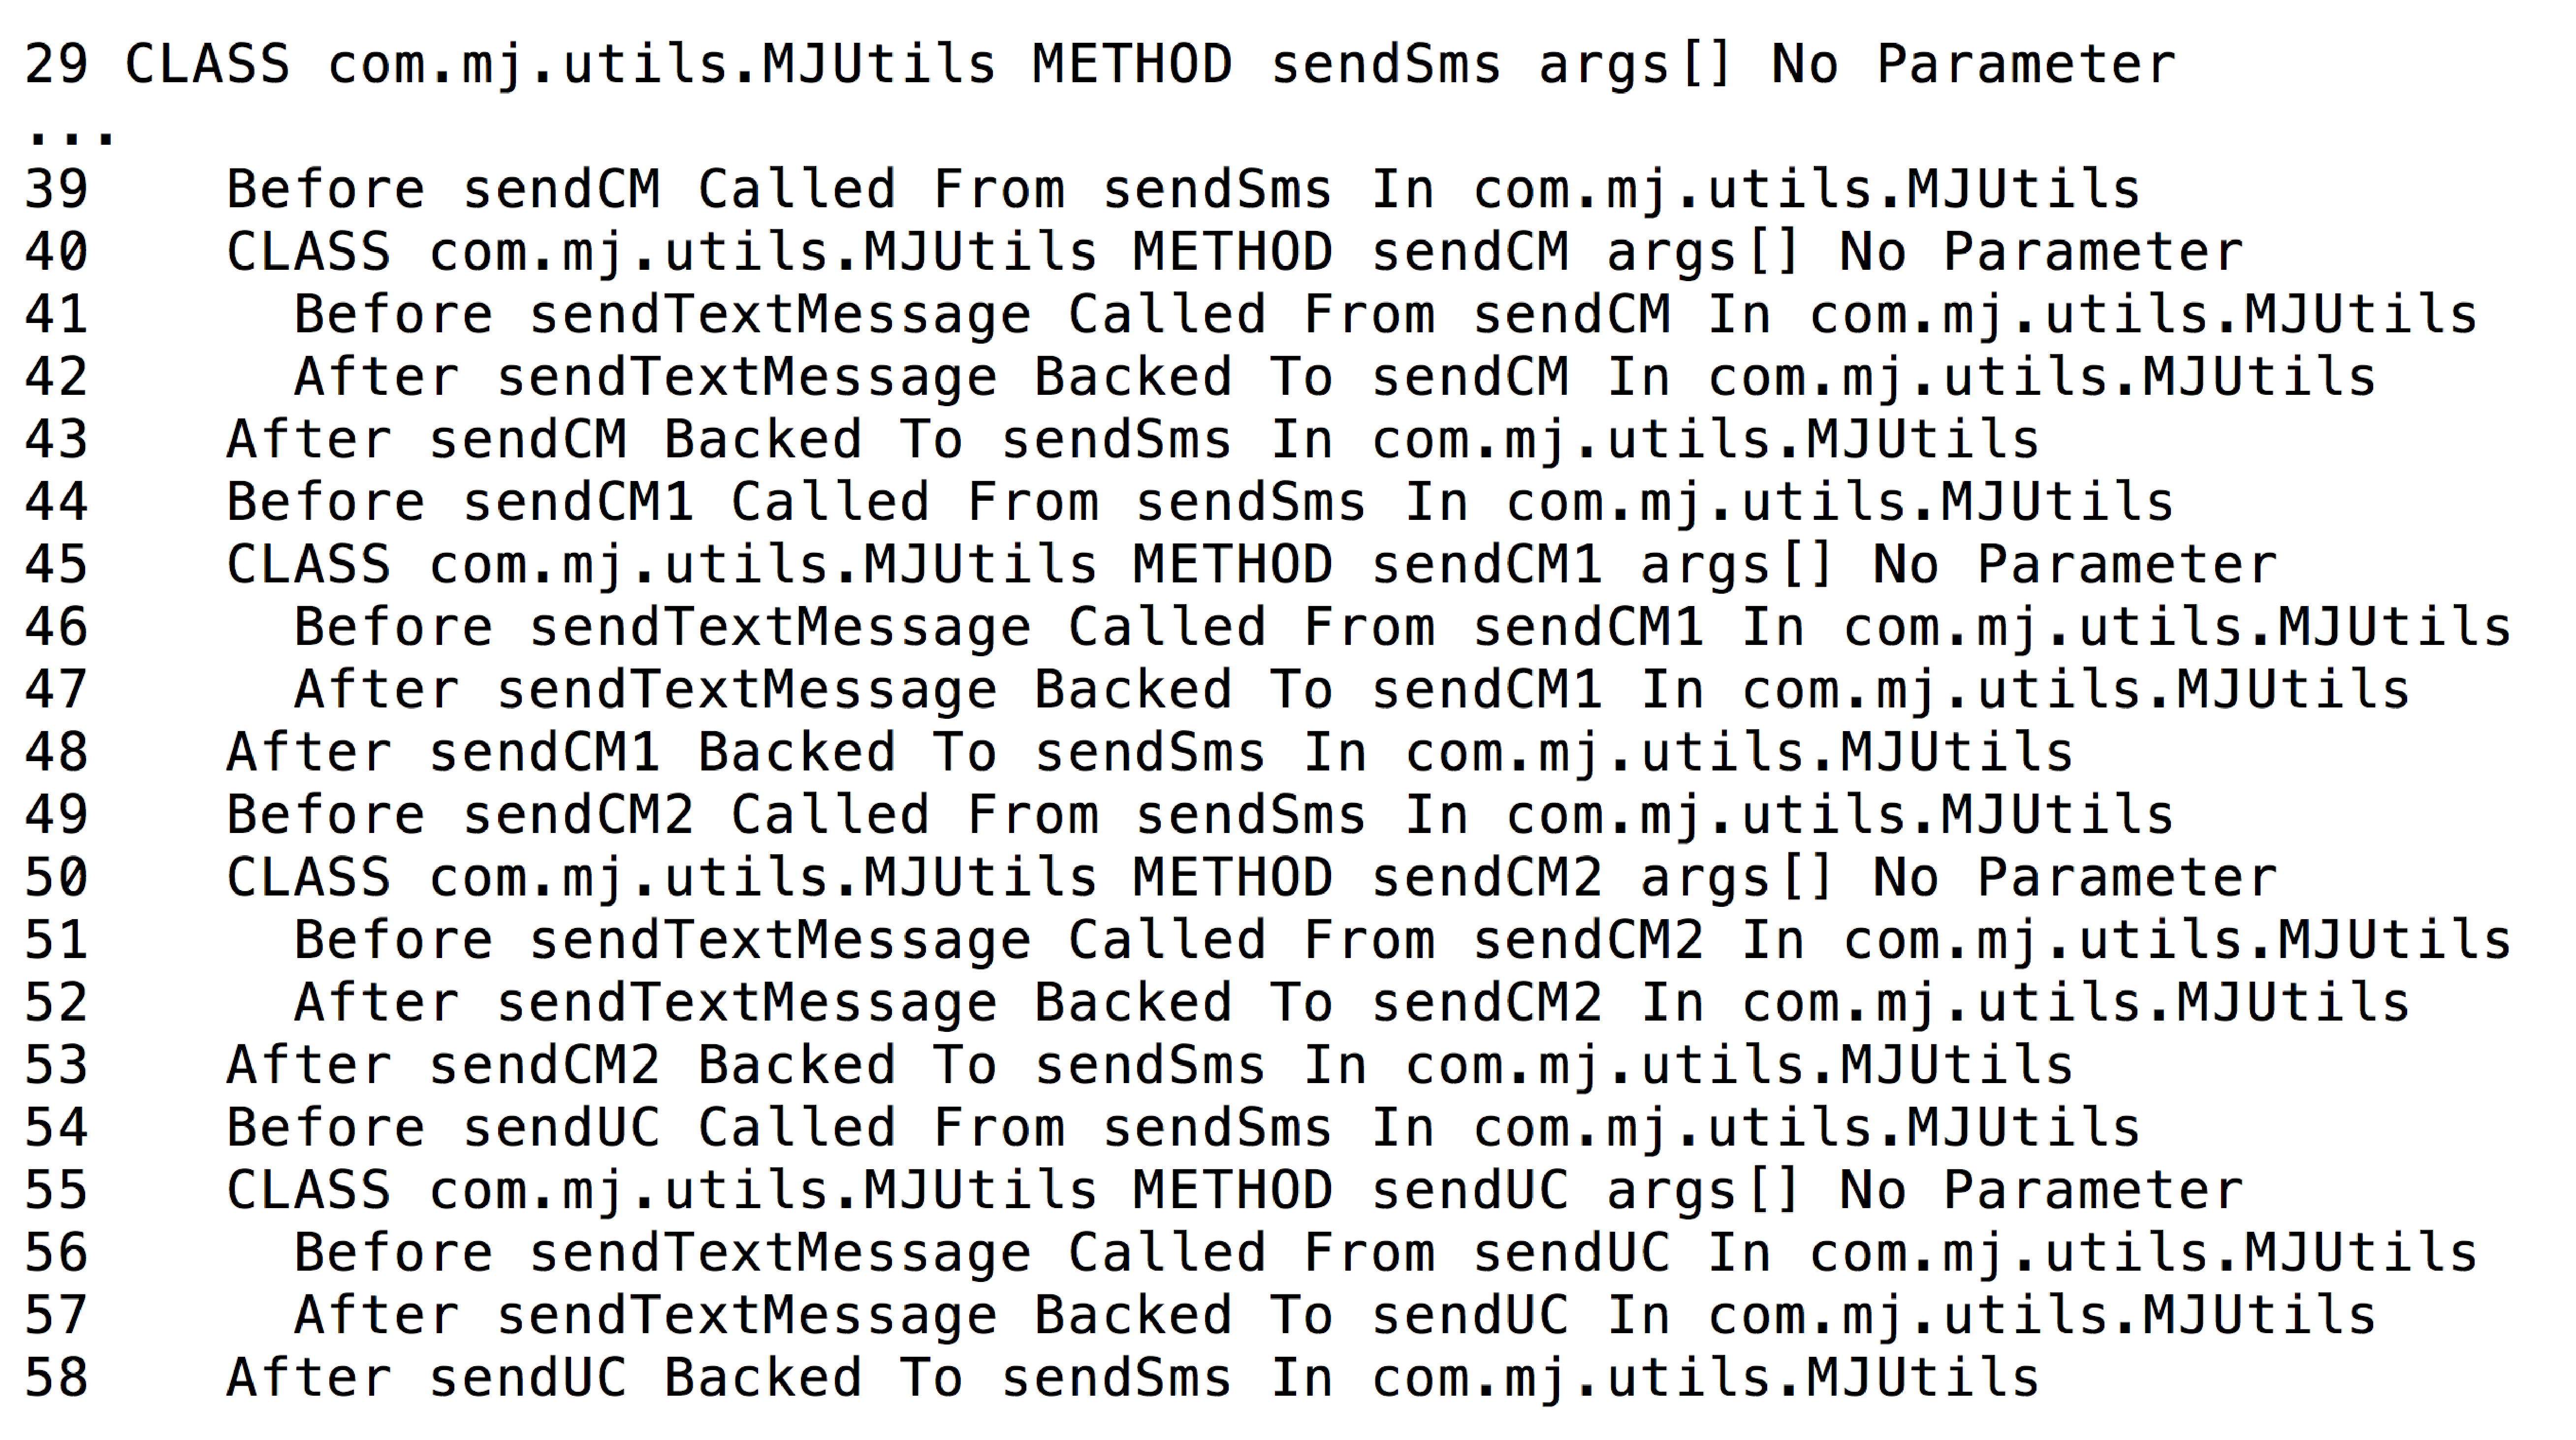
\includegraphics[scale=0.15]{mjutilslog2.eps}
\end{center}
\caption{\ref{private} の手法適用後のcom.mj.utils.MJUtils のログのテキストの一部}
\label{mjutilslog2}
\end{figure}



\begin{figure}[t]
\begin{center}
\graphicspath{{./epsfiles/}}
\includegraphics[scale=0.4]{activity3.eps}
\end{center}
\caption{Activity の遷移}
\label{activity}
\end{figure}


